\documentclass[10pt]{article}
\usepackage[utf8]{inputenc}
\usepackage[margin=0.9in, bottom=0.9in, top=0.9in]{geometry}
\usepackage{graphicx}
\usepackage{float}

% colors
\usepackage[dvipsnames]{xcolor}
\usepackage[citecolor=CadetBlue, linkcolor=CadetBlue, colorlinks=true, urlcolor=CadetBlue]{hyperref}
\definecolor{mygray}{gray}{0.5}
\definecolor{cblue}{RGB}{8, 85, 153}
\definecolor{darkblue}{RGB}{1, 43, 112}
\newcommand{\cblue}[1]{{\textcolor{cblue}{#1}}}
\definecolor{cgreen}{RGB}{8, 153, 83}

\usepackage{titling}
\usepackage{amsmath}
\usepackage{amssymb}
\setlength{\droptitle}{-40pt}

\usepackage[fencedCode,inlineFootnotes,citations,definitionLists,hashEnumerators,smartEllipses,hybrid,underscores=false]{markdown} % for markdown
\usepackage{placeins} %FloatBarrier

\usepackage[hyperpageref]{backref}
% \renewcommand*{\backref}[1]{\ifx#1\relax \else Page #1 \fi}
\renewcommand*{\backrefalt}[4]{%
    \ifcase #1 \footnotesize{(Not cited.)}%
    \or        \footnotesize{(Cited on page~#2.)}%
    \else      \footnotesize{(Cited on pages~#2.)}%
    \fi}
    
\newcommand{\cs}[1]{{\textcolor{cblue}{CS: #1}}}
\usepackage{changepage}


\title{MDCalc Analysis Figures}
\author{}
\date{August 2022}

\begin{document}

\maketitle

Everything here is still rough and potentially needs cleaning before it is fully accurate...

\section{Metadata on CDIs}

Here is some human-labeled metadata on the categorization of different CDIs and their uses. 

\begin{figure}[H]
    \centering
    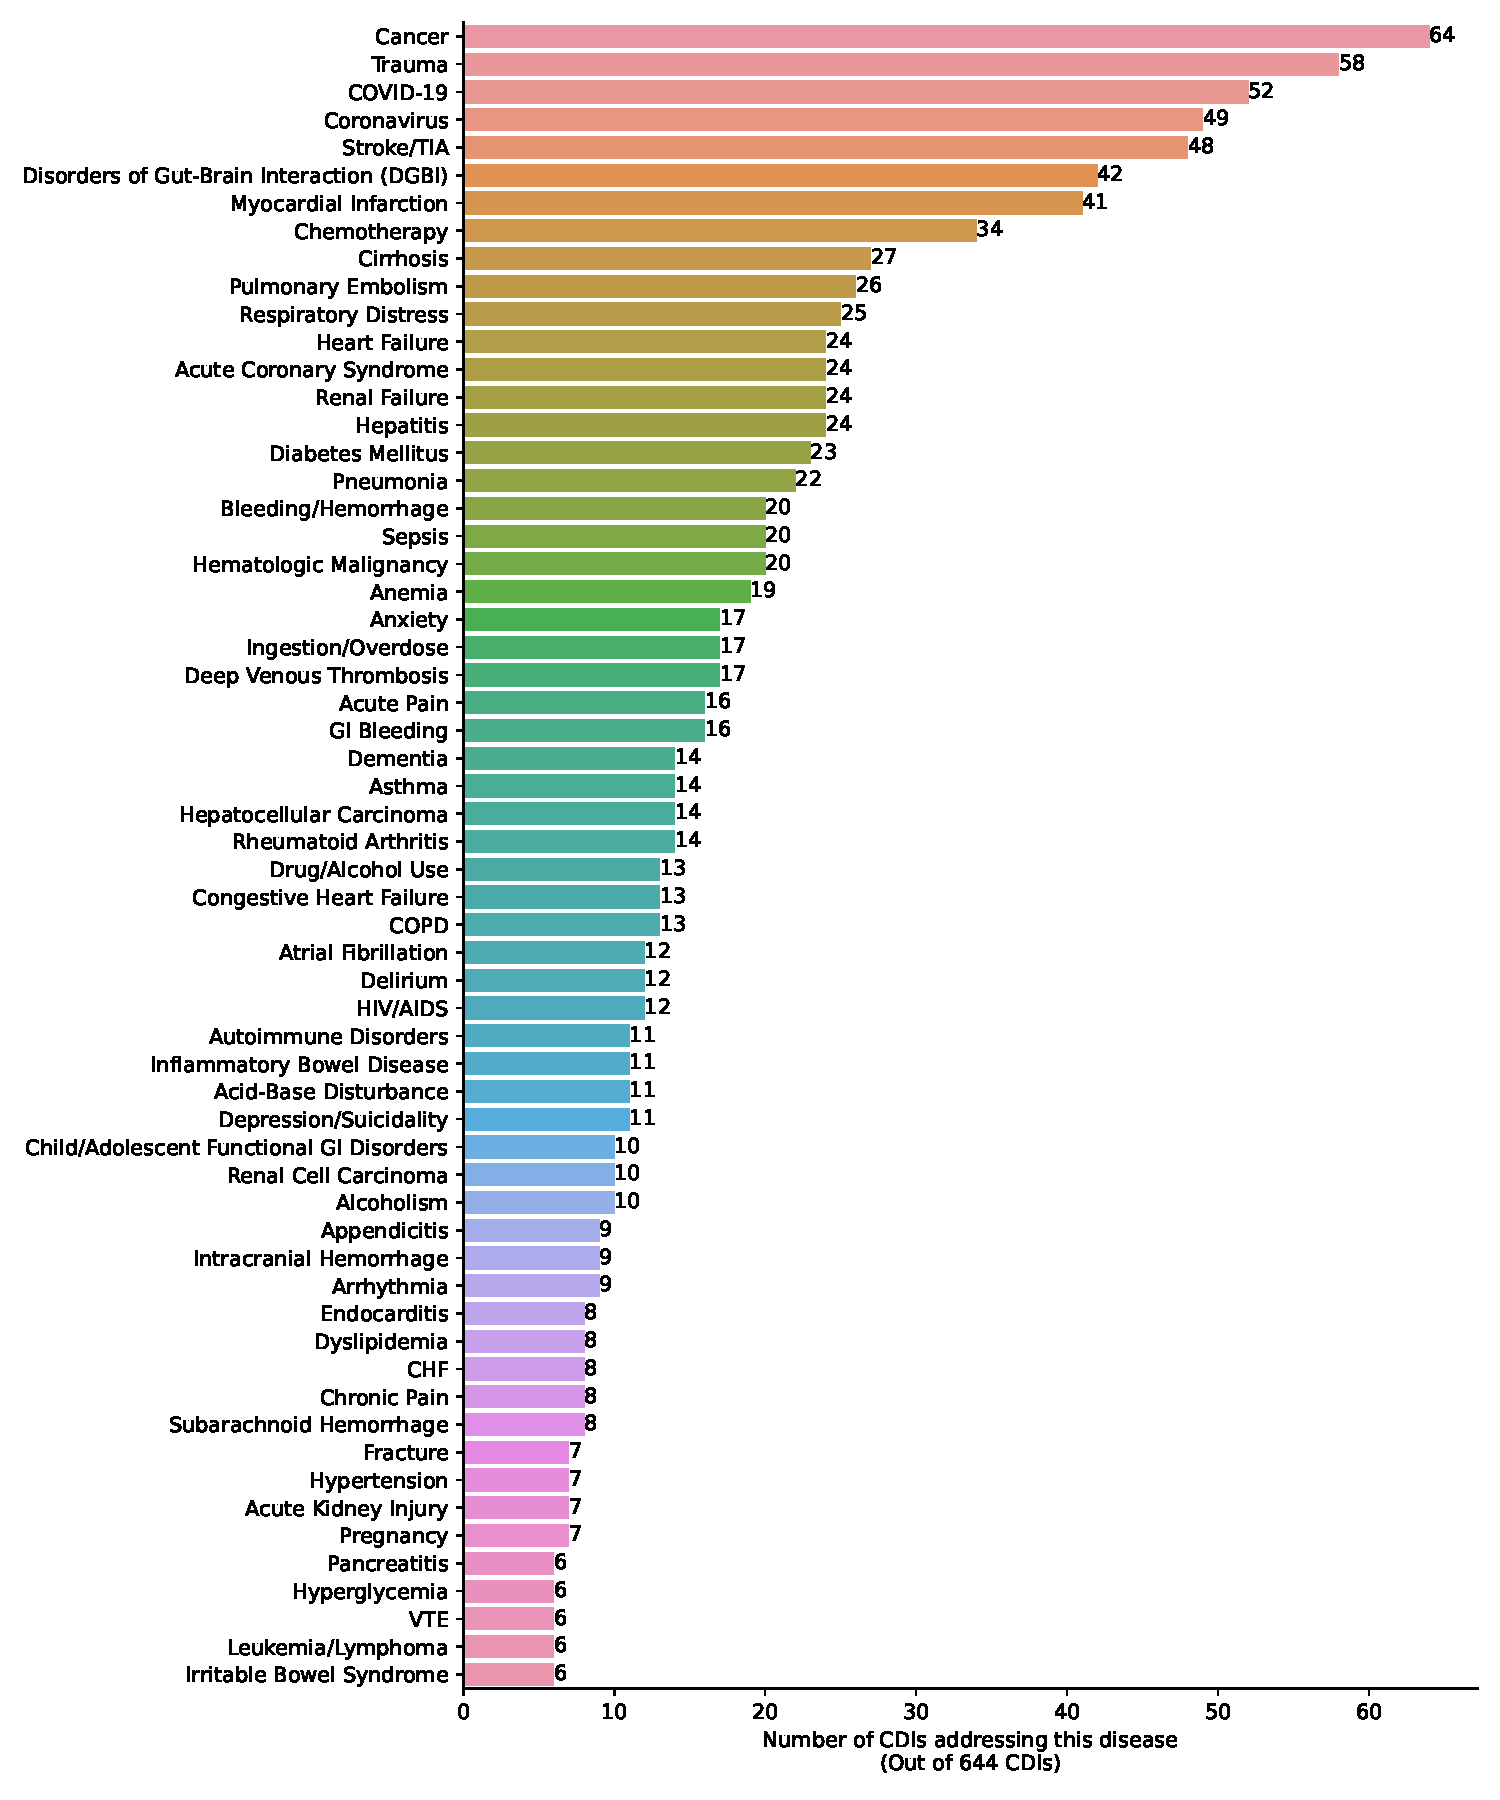
\includegraphics[width=0.49\textwidth]{../results/disease_en.pdf}
    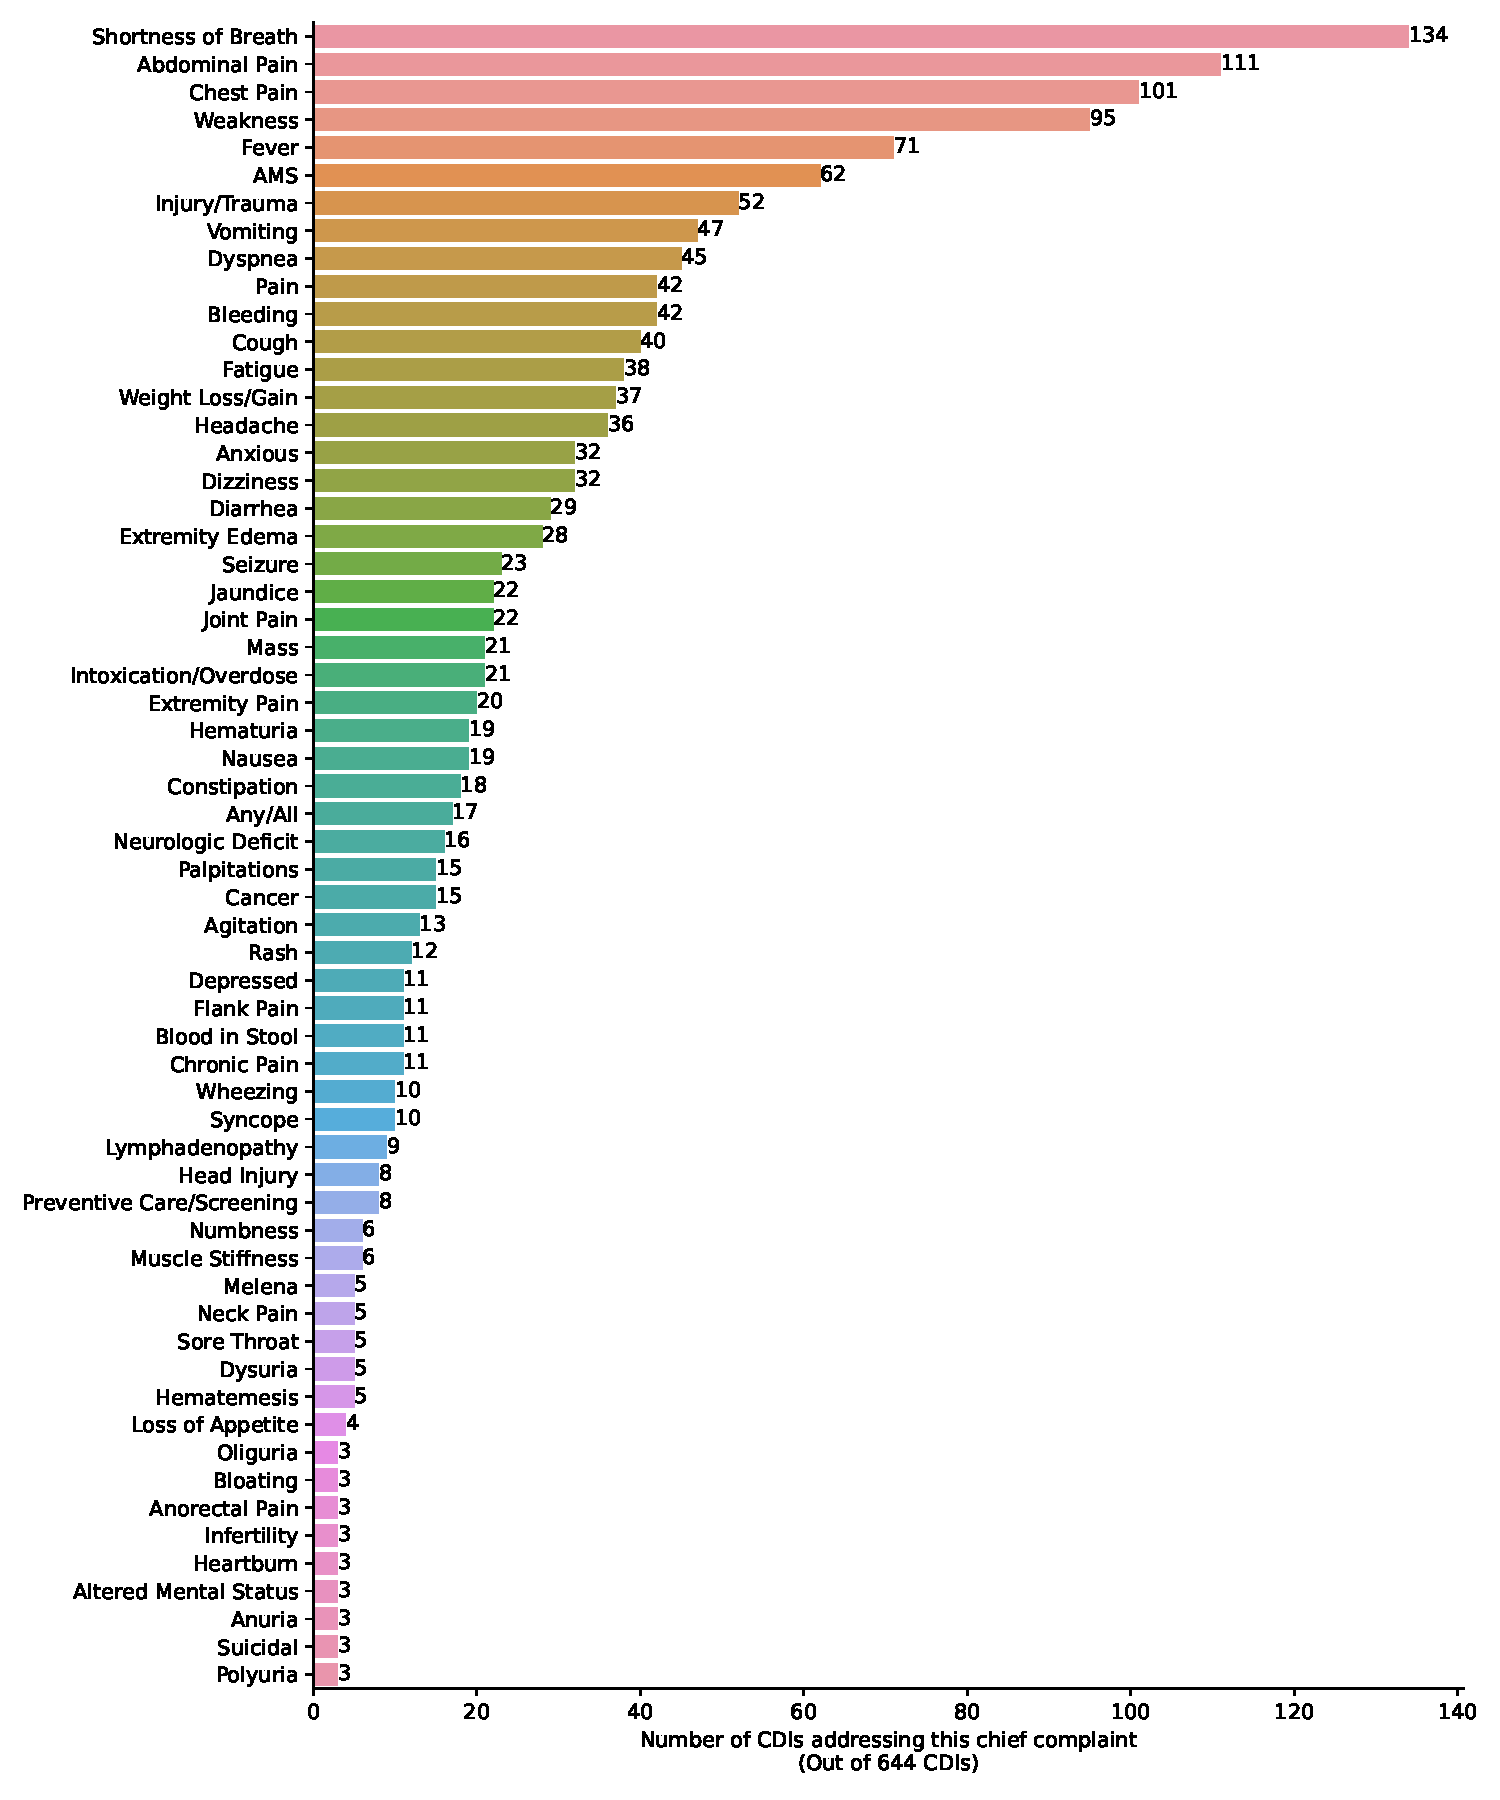
\includegraphics[width=0.49\textwidth]{../results/chief_complaint_en.pdf}
    \caption{Disease and chief complaint.}
\end{figure}

\begin{figure}[H]
    \centering
    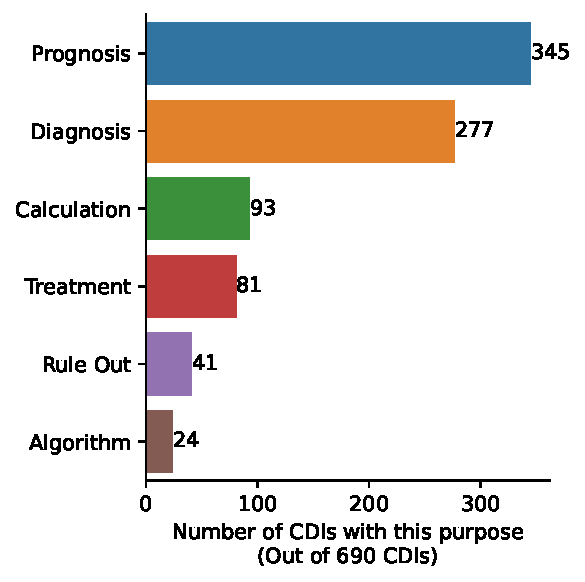
\includegraphics[width=0.49\textwidth]{../results/purpose_en.pdf}
    \caption{Caption}
\end{figure}

\begin{figure}[H]
    \centering
    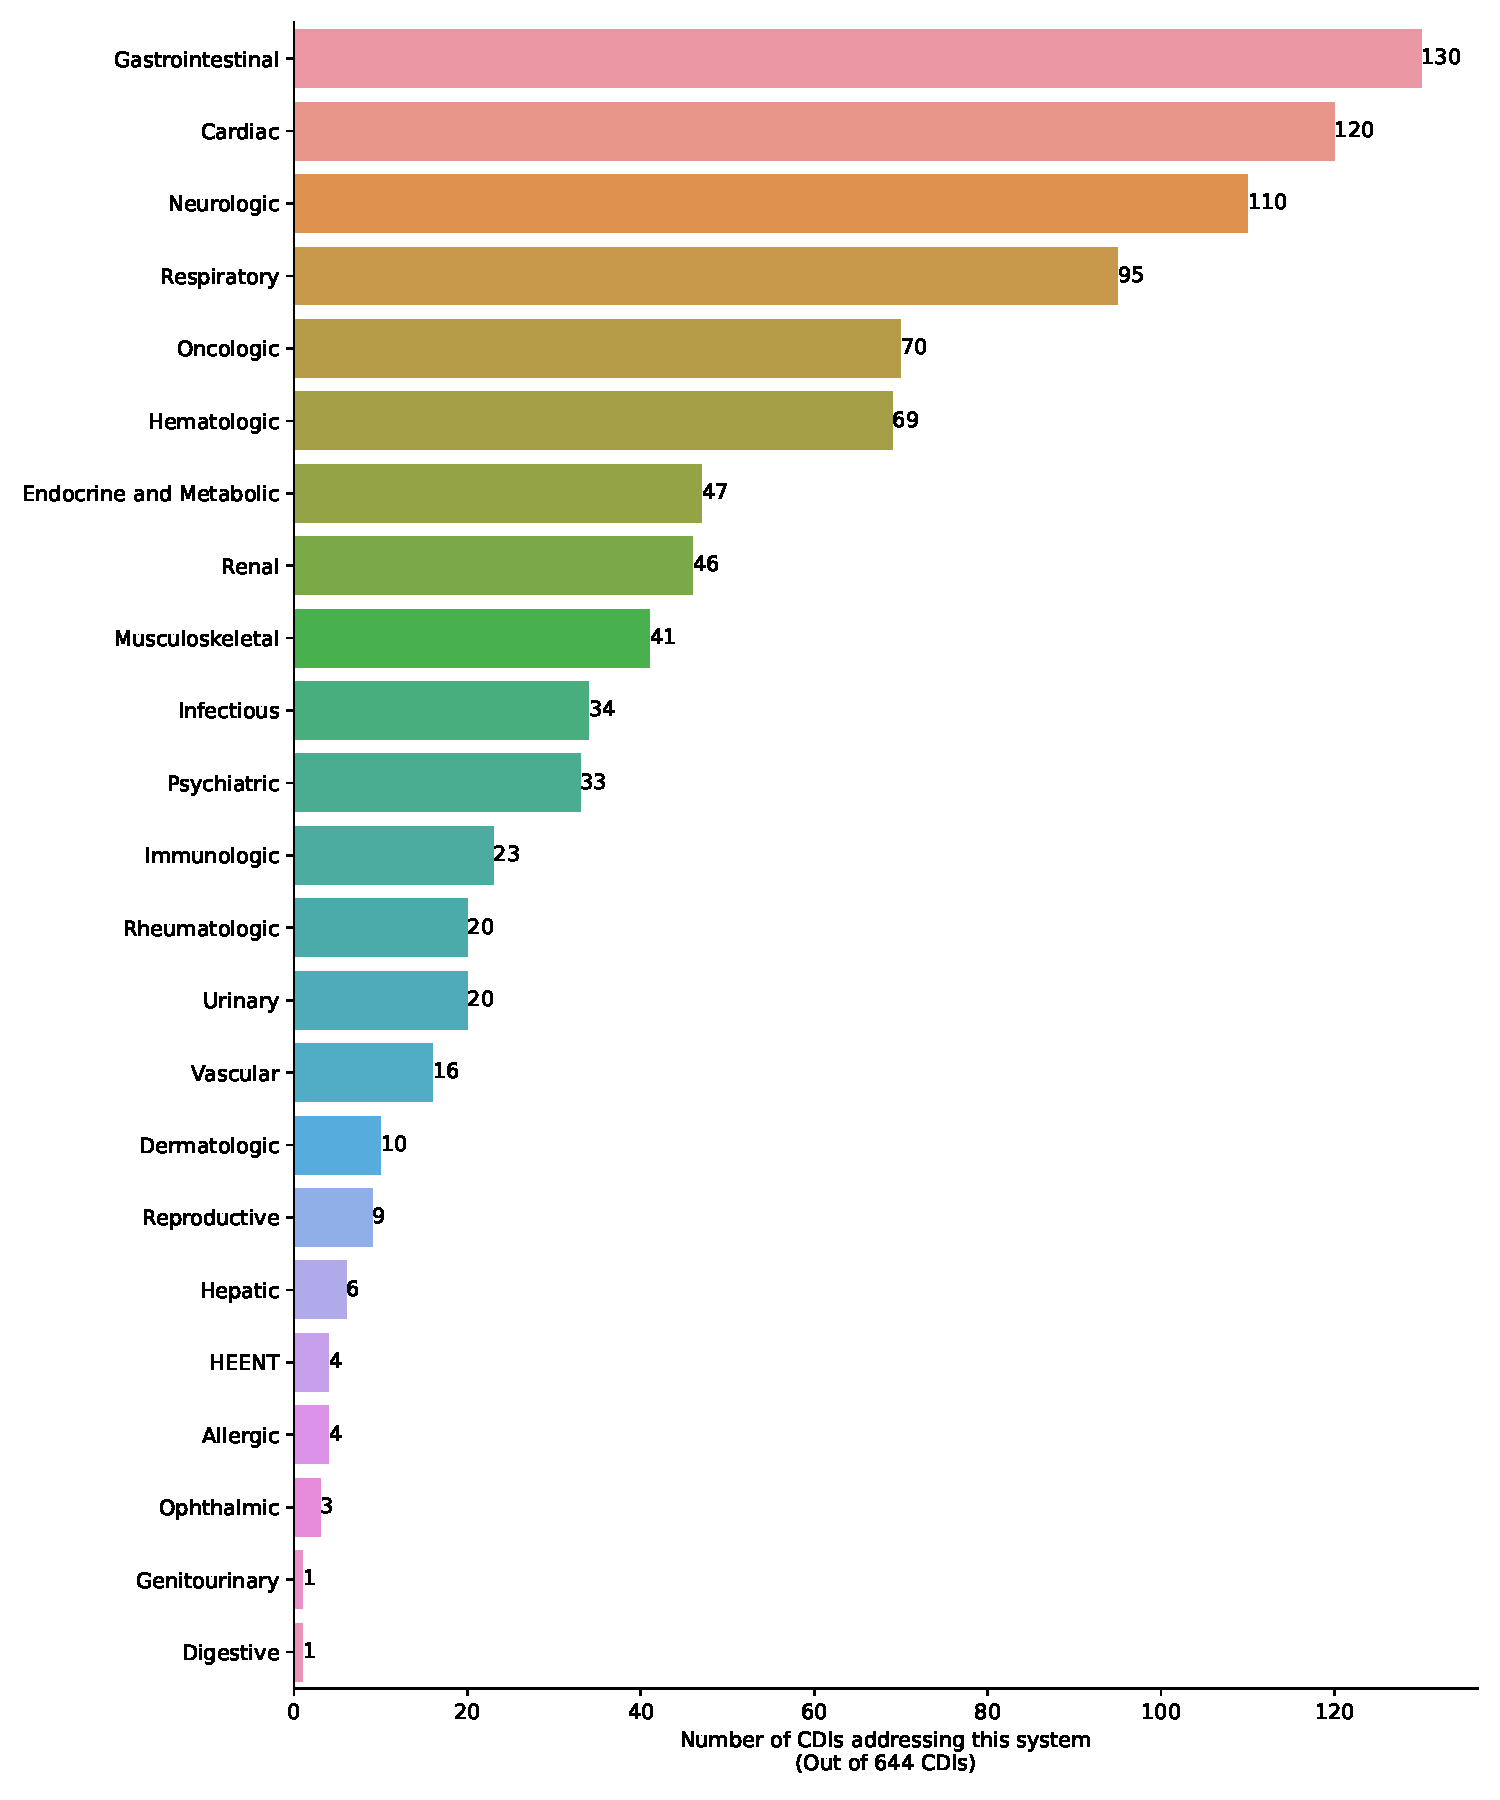
\includegraphics[width=0.49\textwidth]{../results/system_en.pdf}
    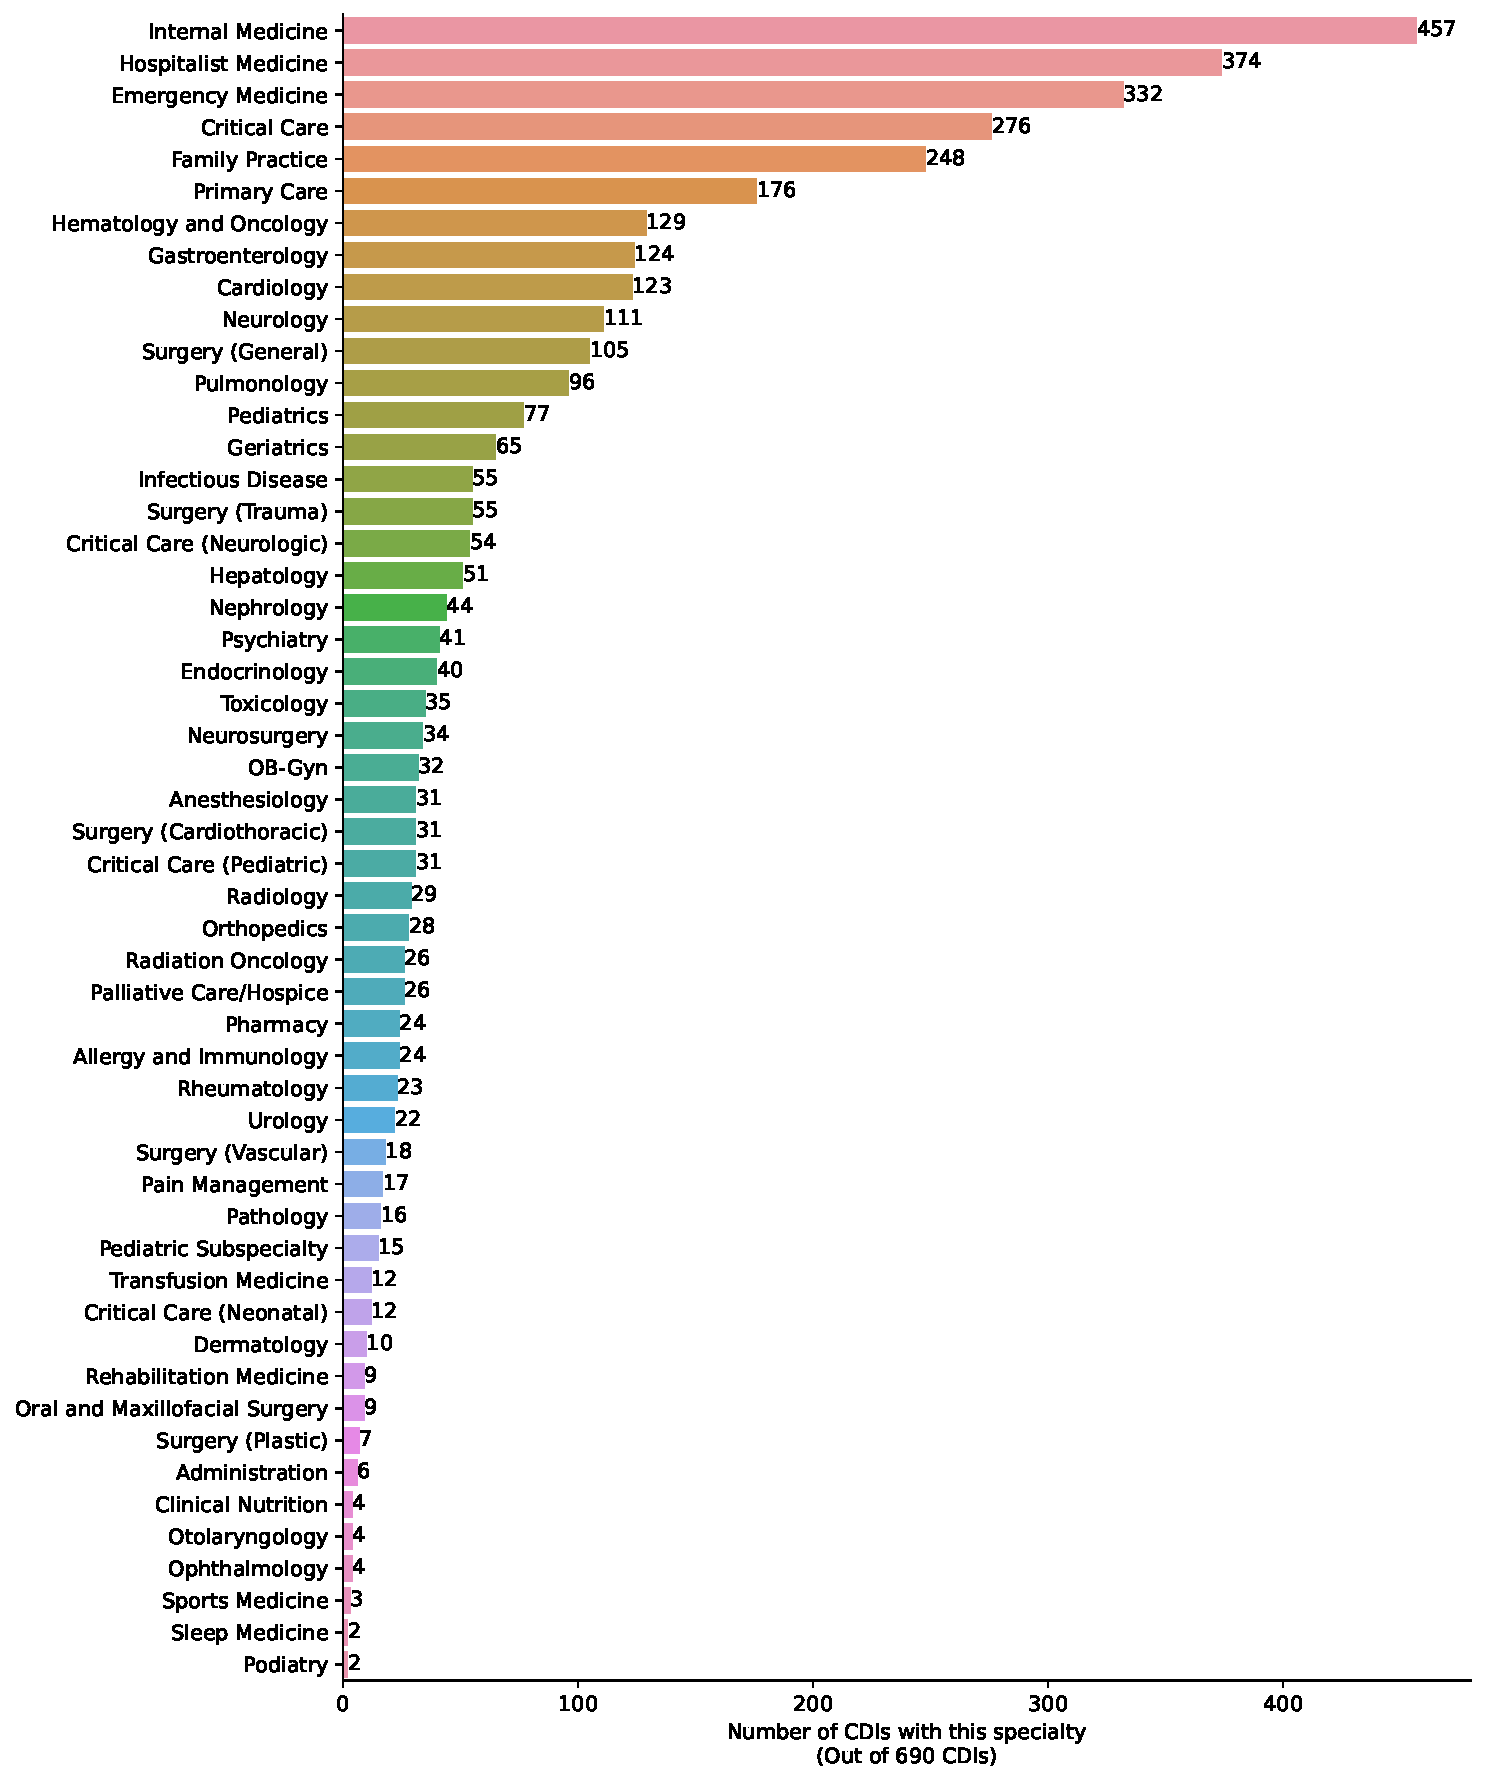
\includegraphics[width=0.49\textwidth]{../results/specialty_en.pdf}
    \caption{System and specialty.}
\end{figure}

\section{Analysis of CDI features}

Here is analysis on the resulting CDIs...

\begin{figure}[H]
    \centering
    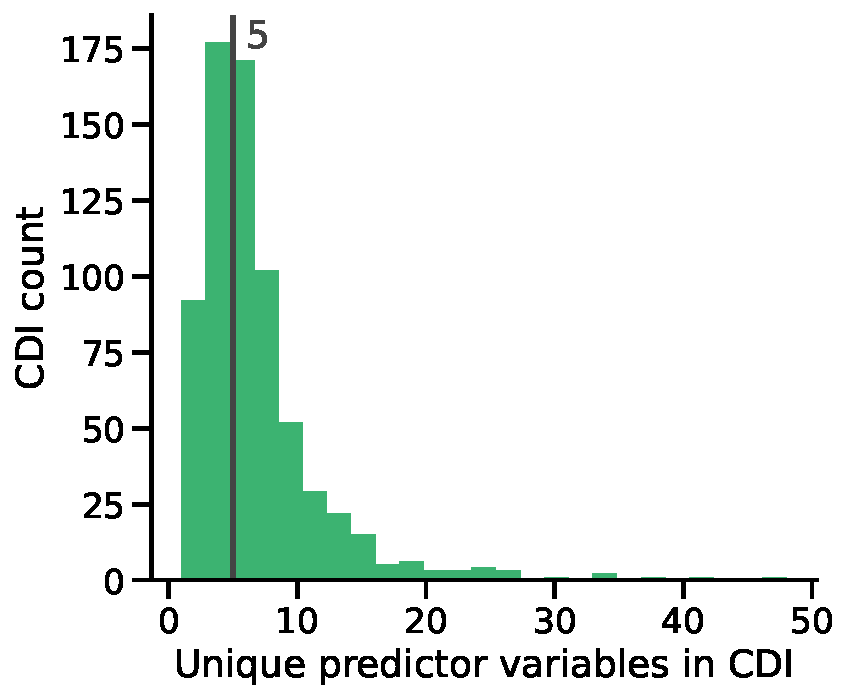
\includegraphics[width=0.49\textwidth]{../results/num_rules_hist.pdf}
    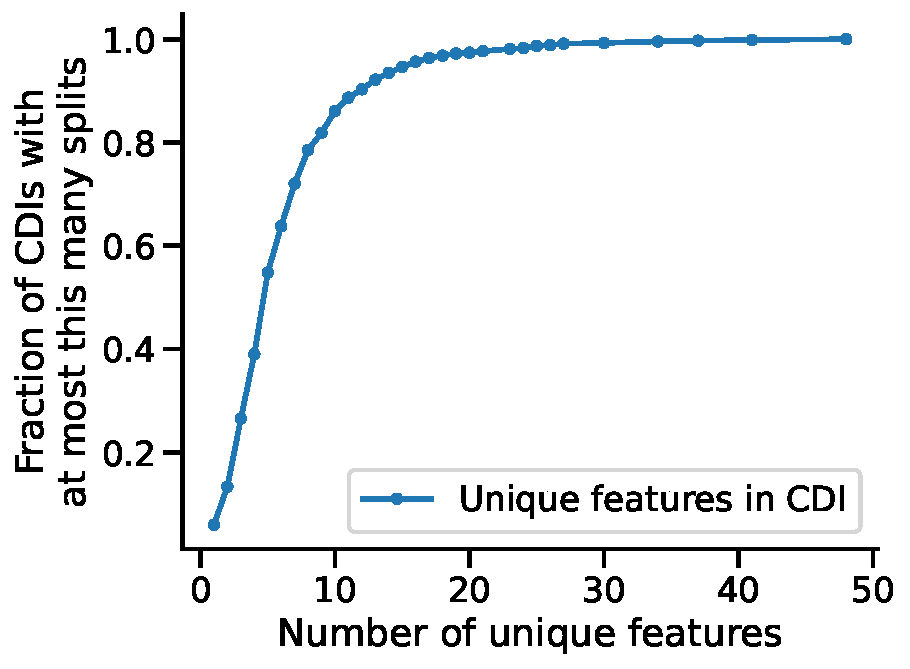
\includegraphics[width=0.49\textwidth]{../results/num_rules_cdf.pdf}
    \caption{Number of splits in each CDI.}
\end{figure}

\begin{figure}[H]
    \centering
    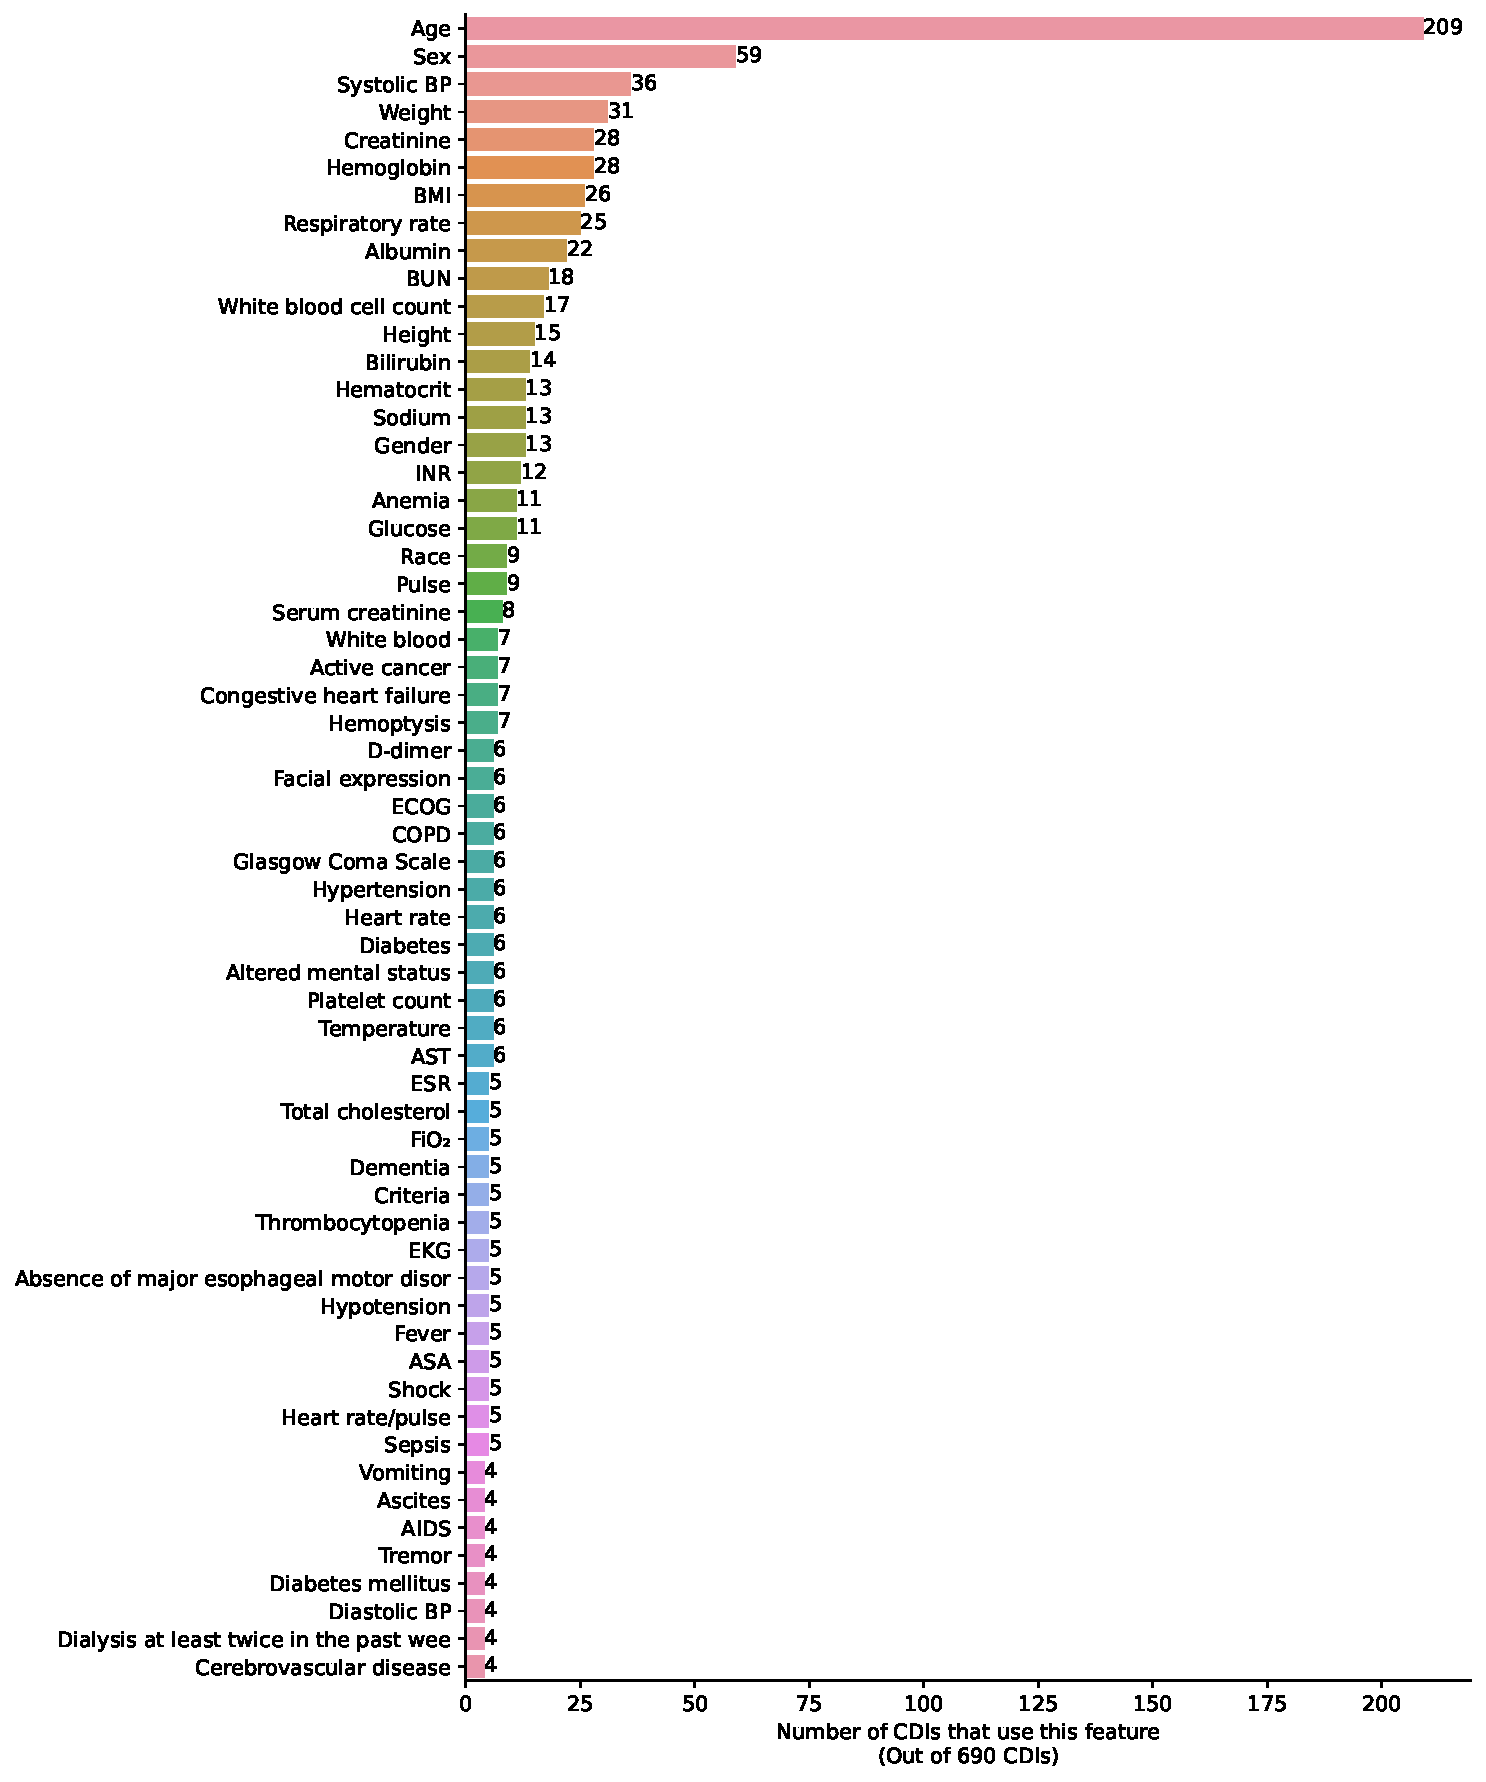
\includegraphics[width=0.65\textwidth]{../results/common_features.pdf}
    \caption{Common features. Age is the most common by far.}
\end{figure}



\end{document}
